\documentclass{standalone}

\usepackage{tikz}
\usetikzlibrary{backgrounds, positioning, decorations.pathreplacing, calc, fit}
\usetikzlibrary{shapes}

\begin{document}

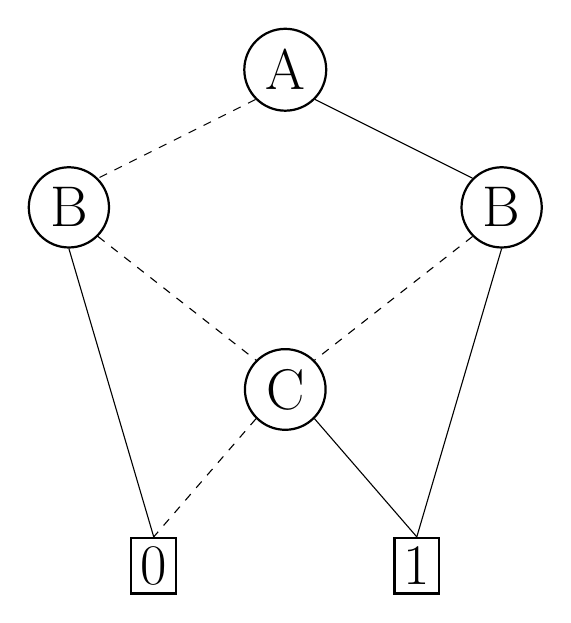
\begin{tikzpicture}
    \tikzstyle{inner} = [draw, circle, thick];
    \tikzstyle{terminal} = [draw, rectangle, thick];

    \node[inner] (A) at (2, 0) {\huge{A}};
    \node[inner, below left = 1 and 2 of A] (Bl) {\huge{B}};
    \node[inner, below right = 1 and 2 of A] (Br) {\huge{B}};
    \node[inner, below = 3 of A] (C) {\huge{C}};

    \node[terminal, below left = 1.5 and 1 of C] (0) {\huge{0}};
    \node[terminal, below right = 1.5 and 1 of C] (1) {\huge{1}};

    \draw[dashed] (A.south west) -- (Bl.north east);
    \draw (A.south east) -- (Br.north west);

    \draw[dashed] (Bl.south east) -- (C.north west);
    \draw (Bl.south) -- (0.north);

    \draw[dashed] (Br.south west) -- (C.north east);
    \draw (Br.south) -- (1.north);

    \draw[dashed] (C.south west) -- (0.north);
    \draw (C.south east) -- (1.north);
\end{tikzpicture}

\end{document}